\documentclass[../main.tex]{subfiles}
 
\begin{document}

Mathematical modelling plays a big role in the description of a large part of phe- nomena in the applied sciences and in several aspects of technical and industrial activity.

By a “mathematical model” we mean a set of equations and/or other mathe- matical relations capable of capturing the essential features of a complex natural or artificial system, in order to describe, forecast and control its evolution. The applied sciences are not confined to the classical ones; in addition to physics and chemistry, the practice of mathematical modelling heavily affects disciplines like finance, biology, ecology, medicine, sociology.

In the industrial activity (e.g. for aerospace or naval projects, nuclear reactors, combustion problems, production and distribution of electricity, traffic control, etc.) the mathematical modelling, involving first the analysis and the numerical simulation and followed by experimental tests, has become a common procedure, necessary for innovation, and also motivated by economic factors. It is clear that all of this is made possible by the enormous computational power now available.

In general, the construction of a mathematical model is based on two main ingredients: general laws and constitutive relations.

In this book we shall deal with general laws coming from continuum mechanics and appearing as conservation or balance laws (e.g. of mass, energy, linear momentum, etc.).

The constitutive relations are of an experimental nature and strongly depend on the features of the phenomena under examination. Examples are the Fourier law of heat conduction, the Fick’s law for the diffusion of a substance or the way the speed of a driver depends on the density of cars ahead.

The outcome of the combination of the two ingredients is usually \textit{a partial differential equation or a system of them}.

\subsection{Partial Differential Equations}

\subsection{Well Posed Problems}

Usually, in the construction of a mathematical model, only some of the general laws of continuum mechanics are relevant, while the others are eliminated through the constitutive laws or suitably simplified according to the current situation. In general, additional information are necessary to select or to predict the existence of a unique solution. These information are commonly supplied in the form of initial and/or boundary data, although other forms are possible. For instance, typical boundary conditions prescribe the value of the solution or of its normal derivative, or a combination of the two, at the boundary of the relevant domain. A main goal of a theory is to establish suitable conditions on the data in order to have a problem with the following features:

\subsection{Basic Facts and Notations}

\subsubsection{Well Posed Problems}

Usually, in the construction of a mathematical model, only some of the general laws of continuum mechanics are relevant, while the others are eliminated through the constitutive laws or suitably simplified according to the current situation. In general, additional information are necessary to select or to predict the existence of a unique solution. These information are commonly supplied in the form of \textit{initial and/or boundary data}, although other forms are possible. For instance, typical boundary conditions prescribe the value of the solution or of its normal derivative, or a combination of the two, at the boundary of the relevant domain. A main goal of a theory is to establish suitable conditions on the data in order to have a problem with the following features:

\begin{enumerate}[nolistsep]
    \begin{easylist2}
        & There exists at least one solution.
        & There exists at most one solution.
        & The solution depends continuously on the data.
    \end{easylist2}
\end{enumerate}

This property is extremely important and may be expressed as a \textbf{local stability of the solution with respect to the data}. Think for instance of using a computer to find an approximate solution: the insertion of the data and the computation algorithms entail approximation errors of various type. A significant sensitivity of the solution on small variations of the data would produce an unacceptable result.

The notion of continuity and the error measurements, both in the data and in the solution, are made precise by introducing a suitable notion of distance. In dealing with a numerical or a finite dimensional set of data, an appropriate distance may be the usual euclidean distance

\subsection{Important Methods and Issues}

\subsubsection{The Method of Characteristics}

\textbf{Subsubsection \ref{sec:4.3.2} / P189, 4.3.2 The method of characteristics, 4.3 Traffic Dynamics, \cite{salsa2016partial}}

To solve the problem, which means to compute the density $\rho$ at a point $(x,t)$ , we follow the idea we already exploited in the linear transport case without external sources:to connect the point $(x,t)$ with a point $(x_0,0)$ on the x-axis, through a curve along which $\rho$ is constant (Fig. \ref{fig:1}).
\\*

\begin{wrapfigure}{\linewidth} \label{fig:1}
\centering
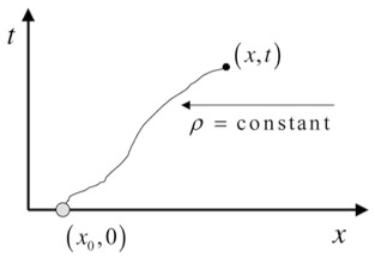
\includegraphics[width=0.4\linewidth]{./PDE1-CharacteristicCurve.png}
    \begin{center}
        \text{Figure \ref{fig:1}, Characteristic Curve}
    \end{center}
\end{wrapfigure}
\\*

Clearly, if we manage to find such a curve, that we call characteristic based at $(x_0,0)$, the value of $\rho$ at $(x,t)$ is given by $\rho (x_0, 0) = g (x_0)$. Moreover, if this procedure can be repeated for every point $(x,t)$, $x \in \mathbb{R}$, $t > 0$, then we can compute $\rho$ everywhere in the upper half-plane and the problem is completely solved. This is the \textit{method of characteristics}.

\subsubsection{Separation of Variables}

\begin{quotebar}
    Mirza Karamehmedović: Many linear PDE problems can be solved using the so-called separation of variables that reduces the PDE problem to a set of ODE problems in the independent variables. This classical method dates back to Fourier (1812), who in fact developed what is now known as Fourier series to solve PDE problems.
\end{quotebar} \\

\textbf{Subsection \ref{sec:2.1.4} / P23, 2.1.4 A solution by separation of variables, \cite{salsa2016partial}}.

\begin{align}
    \begin{cases} \nonumber
    \, U_t - \mathrm{D} U_{xx} = 0 \\
    \, U(x,0) = u^{st}(x) - g(x) \\
    \, U(0,t) = 0 \\
    \, U(L,t) = 0
    \end{cases}
\end{align} \\

\textbf{P269, 5.3.2 Separation of Variables, 5.3 The one-dimensional Wave Equation, \cite{salsa2016partial}}.

\begin{align}
    \begin{cases} \nonumber
        \, u_{tt} - c \, u_{xx} = 0
    \end{cases}
\end{align} \\

\textbf{P303, Square membrane, 5.7.1 Small vibrations of an elastic membrane, 5.7 Two Classical Models}

Problem 3, Assignment 4: Solve the inital-boundary problem with wave equation:
\begin{align}
    \begin{cases} \nonumber
        \, u_{tt} - 9 \, \left(\cfrac{\partial^2 u}{\partial x^2} + \cfrac{\partial^2 u}{\partial y^2}\right) = 0 \text{ ,  } 0 < x < 3 \text{ ,  } 0 < y < 2 \text{ ,  } t > 0 \\
        u(x, y, 0) = - \sin{(2 \, \pi \, x)} \, \sin{\left(\cfrac{\pi}{4} \, y \right)} \text{ ,  } 0 \leqslant x \leqslant 3 \text{ ,  } 0 \leqslant y \leqslant 2 \\
        u_t(x, y, 0) = \sin{\left(\cfrac{\pi}{3} \, x \right)} \, \sin{\left(\cfrac{7 \, \pi}{4} \, y \right)} \text{ ,  } 0 \leqslant x \leqslant 3 \text{ ,  } 0 \leqslant y \leqslant 2 \\
        u(0, y, t) = u(3, y, t) = 0 \text{ ,  } 0 \leqslant y \leqslant 2 \text{ ,  } t \geqslant 0 \\
        u(x, 0, t) = 0 \text{ ,  } 0 \leqslant x \leqslant 3 \text{ ,  } t \geqslant 0 \\
        u_y(x, 2, t) = 0 \text{ ,  } 0 \leqslant x \leqslant 3 \text{ ,  } t \geqslant 0
    \end{cases}
\end{align}

\subsubsection{The Global Cauchy Problem}

In important applications, for instance in financial mathematics, x varies over unbounded intervals, typically $(0, \infty)$ or $\mathbb{R}$. In these cases one has to require that the solution does not grow too much at infinity. \\

\textbf{Section \ref{sec:2.8} / P76, 2.8.1 The homogeneous case, 2.8 The Global Cauchy Problem, 2 Diffusion, \cite{salsa2016partial}}.

Problem B, Assignment 2: Consider the global Cauchy problem:
\begin{align}
    \begin{cases}
        \, u_t - u_{xx} = 0 \quad & x \in \mathbb{R} \text{ ,  } t > 0 \\
        \, u(x,0) = g_u(x) = 3 \, \cos{x} \quad & x \in \mathbb{R}
    \end{cases}
\end{align} \\

\textbf{P275, 5.4.1 The homogeneous equation, 5.4 The d'Alembert Formula, 5 Waves and Vibrations, \cite{salsa2016partial}}, the equation in the book:
\begin{align}
    \begin{cases} \nonumber
        \, u_{tt} - c^2 \, u_{xx} = 0 \quad \text{ ,  } x \in \mathbb{R} \text{ ,  } t > 0\\
        \, u(x, 0) = g(x) \quad \text{ ,  } x \in \mathbb{R} \\
        \, u_t(x, 0) = h(x)\quad \text{ ,  } x \in \mathbb{R}
    \end{cases}
\end{align}

Problem 2, Assignment 4: Assume a function $u(x, t)$ is in $C^2(\mathbf{R} \times [0, \infty[)$, and satisfies:
\begin{align}
    \begin{cases} \nonumber
        \, u_{tt} - 4 \, u_{xx} = 0 \\
        \, u(x, 0) = g(x) \\
        \, u_t(x, 0) = h(x) 
    \end{cases}
\end{align}
which is a Cauchay-Dirichlet problem with a wave equation, and
\begin{align}
    g(6) &= 6 \nonumber \\
    g(2) &= 8 \nonumber \\
    \int_0^2 \, h(y) \, \mathrm{d} y &= - 12 \nonumber \\
    \int_0^6 \, h(y) \, \mathrm{d} y &= 8 \nonumber
\end{align} \\

\textbf{P310, 5.8 The Global Cauchy Problem, 5 Waves and Vibrations, \cite{salsa2016partial}}, the equation in the book:
\begin{align}
    \begin{cases} \nonumber
        \, u_{tt} - c^2 \, \Delta u = 0 \quad \text{ ,  } \vec{x} \in \mathbb{R}^3 \text{ ,  } t > 0\\
        \, u(\vec{x}, 0) = g(\vec{x}) \quad \text{ ,  } \vec{x} \in \mathbb{R} \\
        \, u_t(\vec{x}, 0) = h(\vec{x})\quad \text{ ,  } \vec{x} \in \mathbb{R}
    \end{cases}
\end{align} \\

\subsubsection{Well-posed Problem and Uniqueness}

As mentioned in P5, 1.3 Well posed problem, \cite{salsa2016partial}, the governing equations in a mathematical model have to be supplemented by additional information in order to obtain a well posed problem, i.e. a problem that has exactly one solution, depending continuously on the data. \\

\textbf{Subsubsection \ref{sec:2.1.3} / P20, 2.1.3 Well posed problems $(n = 1)$, 2.1 The Diffusion Equation}. \\

\textbf{Subsection \ref{sec:3.2} / P116, 3.2 Well Posed Problems. Uniqueness, 3 The Laplace Equation, \cite{salsa2016partial}} \\

\textbf{P298, 5.6.2 Well posed problems. Uniqueness, 5.6 The Multi-dimensional Wave Equation $(n > 1)$, \cite{salsa2016partial}}.



\end{document}